\section{Approach} \label{Sec:approach}
\begin{figure}[!t]
  \centering
  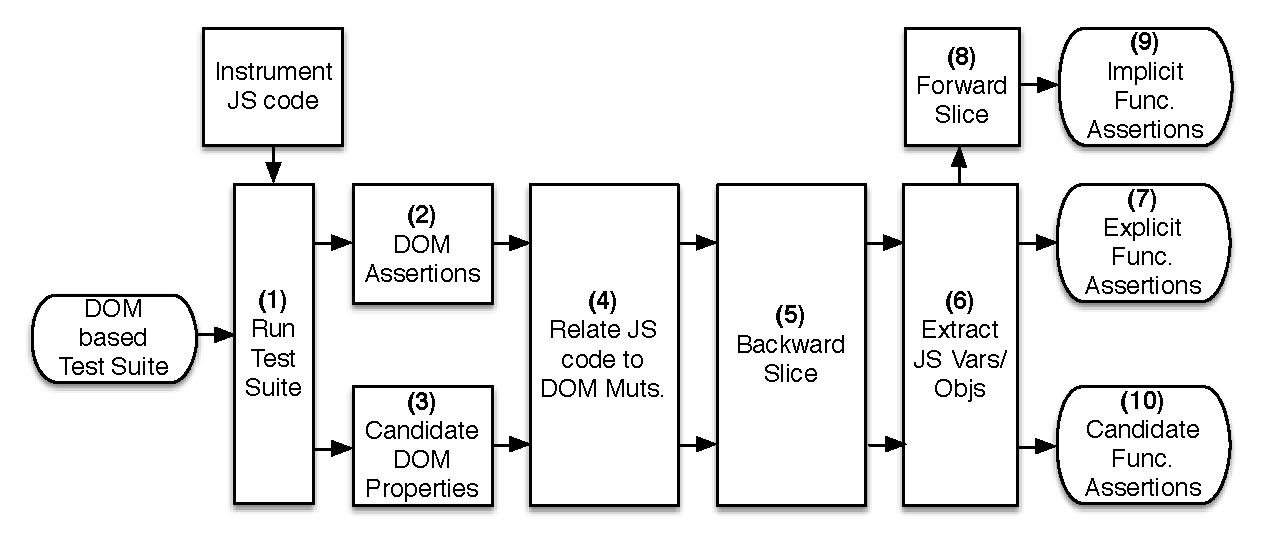
\includegraphics[width=1\hsize]{fig/approachDiagram}
 % \vspace{-0.2in} 
  \mycaption{Overview of our assertion generation approach.}
  \label{Fig:approachDiagram}
 % \vspace{-0.2in} 
\end{figure}
\IncMargin{0em}
\begin{algorithm}[t]
{\scriptsize
\SetKwInOut{Input}{input}\SetKwInOut{Output}{output}
\Input{Test suite $T$; The set of test cases $tc_i \in T$}
\Output{The ordered set of oracles $oracles$}
\BlankLine

\Begin {
\nl \For{$tc_i \in T$}{
\nl  $trace \leftarrow textsc{Exec}(tc_i)$\\
\nl  $domAccss \leftarrow \textsc{GetDOMAcc}(trace)$\\   	
\nl  $freqAccdDOM\leftarrow \emptyset$\\
\nl  \For{$dom \in domAccss $}{
\nl   \If{$\textsc{DOMUsgFreq}(dom) \geq \frac{1}{NoOfDOMElems} $}{
\nl    $freqAccdDOM \leftarrow dom \cup freqAccdDOM$\\       
      }
     }
\nl  \For{$asstn \in assertions_{tc_i}$}{
\nl   $asserDOMAcc \leftarrow \textsc{GetDOMAcc}(asstn)$\\
\nl   $asserDOMMuts \leftarrow \textsc{GetDOMMuts}(asserDOMAcc)$\\
\nl   \For{$domMut \in asserDOMMuts$}{
\nl    $bwSts \leftarrow \textsc{GetBWSlice}(domMut, trace)$\\
\nl    $asstnRel \leftarrow \textsc{GetWrVars}(bwSts)$\\
\nl    $potAsstnRel \leftarrow \textsc{GetFWSlice}(asstnRel, trace)$\\
      }
     }
\nl  $nonAsserDOMMuts \leftarrow \textsc{GetDOMMuts}(freqAccdDOM)$\\
\nl  \For{$domMut \in nonAsserDOMMuts$}{
\nl   $bwSts \leftarrow \textsc{GetBWSlice}(domMut, trace)$\\
\nl   $nonAsstnRel \leftarrow \textsc{GetWrVars}(bwSts)$\\
     }
\nl  $asstnRelOrcls[func]_{f=1}^{n} \leftarrow \textsc{GetValue}(\textsc{Accessibles}([func]_{f=1}^{n}, asstnRel))$\\
\nl  $candidOrcls[func]_{f=1}^{n} \leftarrow \textsc{Accessibles}([func]_{f=1}^{n}, [potAsstnRel \cup nonAsstnRel])$\\
\nl  $oracles[func]_{f=1}^{n}.\textsc{Add}(asstnRelOrcls \cup candidOrcls)$\\
   }
\nl $\textsc{Rank}(oracles[func]_{f=1}^{n})$\\
\nl return $(oracles[func]_{f=1}^{n})$
}
\caption{Oracle Generation} 
\label{Alg:algorithm}
}
\end{algorithm}
%\DecMargin{lem}
\figref{approachDiagram} shows an overview of our unit-level assertion generation technique.
At a high level, our approach generates code-level assertions based on human written DOM-based tests and assertions. Our code level assertions fall in the following three categories: (1) explicit assertions, which are directly inferred from analyzing the manually written DOM-based assertions, (2) implicit assertions, which are indirectly affected by the human written DOM-based assertions, and (3) candidate assertions, which are not considered in the written DOM-based assertions, yet are potentially useful for fault detection. We describe how our approach below finds the three categories of assertions. The numbers below in parentheses correspond to those in the boxes of \figref{approachDiagram}.

In the first part of our approach we (1) execute the instrumented application by running the existing DOM-based test suite, and gather a detailed execution trace of the application. We then extract (2) DOM-based assertions, and (3) candidate DOM element properties, which are useful DOM properties that can be used to generate assertions. We also (4) identify the initial point of connection between the application's source code and checked DOM element. 
%We collect lines of code responsible for updating the corresponding DOM element. 
%We determine DOM mutating statements, 

In the second part of our approach, we use the information gathered in the first part to obtain the assertions. In this part, we
 (5) calculate the backward slice of the DOM mutating statements to find the entire code blocks that update the checked DOM element, (6) extract accessible entities from the obtained statements, and (7) form explicit assertions using the accessible entries. 
 We further (8) perform a forward slice on the extracted entities to identify statements that are implicitly affected by such entities, and (9) form implicit assertions using the collected entities, and (10) generate candidate assertions by performing steps (4), (5), and (6) on the inferred candidate DOM element properties (3).

Our overall unit-level assertion generation is presented in \algref{algorithm}. In the following sections we describe our technique for extracting DOM related information from the execution (\secref{extractDomRelatedInfo}), relating
DOM mutations to the \javascript code (\secref{domToCode}), and generating unit test assertions (\secref{unitLevelAssertion}).   
\subsection{Extracting DOM-Related Characteristics} \label{Sec:extractDomRelatedInfo}
The DOM connects a test case to the web application's code. Therefore, we first need to analyze the DOM-based test suite and extract the following pieces of information: (1) DOM-related operations of the existing test suite that may have tight connection with the \javascript code, and (2) frequently accessed DOM properties, which potentially are potentially influential in improving the fault finding capability of the test suite, but left unchecked in the manually-written test suite.
\headbf{DOM-Related Operations}
Any written test case needs to check the correctness of the application's behaviour. In a DOM-based test case the expected behaviour is checked through DOM-based assertions.
DOM-based assertion is defined as $<DOMProp,ExpVal>$, where $DOMProp$ is a DOM element feature (e.g. attribute, and/or textual value), and $ExpVal$ is the correct value expected by the assertion. Through the rest of the paper, we call DOM element feature as DOM property. 
DOM-based assertions play a significant role in our approach as they can guide us towards important portions of the underlying \javascript code that need to be checked in unit-level assertions.

For each DOM-based assertion we find \emph{Intra DOM assertion correlation} within the test suite.
\begin{mydef}[Intra DOM Assertion Correlation]
An intra DOM asseetion correlation is defined as a three tuple of $<DOMProp, AccDOM, AccDOMDep>$, where $DOMProp$ is the accessed DOM property within the assertion, $AccDOM$ is the accessed DOM elements in the test case pertaining to the assertion, and $AccDOMDep$ is the DOM dependencies of the assertion in the test case.
\end{mydef}
\textsc{GetDomAcc} in line 10 of \algref{algorithm} retrieves DOM dependencies of the assertion in the test case.
%, we instrument the test case by wrapping around method calls that accesses DOM elements.
Going back to our example in \figref{example}(b), tracking the assertion in line 11 shows that it has a DOM dependency to a \code{div} element with class \code{shopContainer}, which is accessed in line 10.

We further need to link the inferred Intra DOM assertion correlation with the application's code.
We call the correlation between the DOM-based assertion and the \javascript code of the application as \emph{inter DOM assertion correlation}.
\begin{mydef}[Inter DOM Assertion Correlation]
An inter DOM assertion correlation is defined as\\
$<AccDOMDep, InitCode>$, where $InitCode$ is the initial point of contact in the application's code segment, that is responsible for mutating $AccDOMDep$ the previously extracted DOM elements from the test suite.
\end{mydef}
To infer this type of correlation we track DOM's evolution of the $AccDOMDep$ (\textsc{GetDomMuts} in line 13 of the algorithm) as well as invoked event handlers as the test case runs. 
We consider additions and removals of child nodes, changes to attributes, and updates to child text nodes as DOM mutations. For instance, running the sample test case in \figref{example}(b) results in mutating (1) the textual value of \code{div} element with class \code{shopContainer}.
%We call the correlation between the DOM-based assertion and the \javascript code of the application as \emph{inter DOM assertion correlation}. This correlation is defined as $<AccDOMDep, InitCode>$, where $InitCode$ is the initial point of contact in the application's code segment, that is responsible for mutating the previously extracted DOM elements from the test suite ($AccDOMDep$).  
%We make use of \code{document.onload} event to log the initial DOM state. 
%An observer module is then used to monitor mutations on the DOM during the test case execution. 
%In addition to DOM changes, we also keep track of \javascript events as well as invoked event handlers. This information is later used to find the initial point of contact between a DOM mutation and the executed code segments.
%For instance, running the sample test case in \figref{example}(b) results in mutating (1) the textual value of \code{div} element with class \code{shopContainer}, and (2) the \code{class} attribute of DOM element with ID \code{couponButt}.
\headbf{Frequently Accessed DOM Properties}
In addition to DOM-based assertions, we further consider DOM element properties, that are frequently accessed within the application as the test case runs (lines 1 to 7 of \algref{algorithm}). 
\textsc{Acc} in line 6 of the algorithm computes the access frequency of a DOM property, $freqAccdDOM$ in line 7 contains the inferred candidate DOM properties, and \textsc{GetDomMuts} in line 19 records DOM mutations occur
on candidate DOM properties.
The intuition is that frequent use of a given DOM property can point to the extent of application's behaviour dependency on the DOM property. Thus, if changes happen to that property through the \javascript code, it is important to assert the correctness of such mutations. We define the access frequency of a DOM element property as the number of times that the element's property has been read during the execution of a test case. DOM properties include attributes as well as textual value of the elements.
In order to record DOM property accesses within the application, we rewrite native function calls used by programmers to access DOM element such as \code{getElementById}, \code{getElementsByClassName}, and/or \code{getElementsByTagName}. The returned object from these functions is later used to access attributes or textual values of the element. Thus, we apply a forward slice on the returned object to find instances of element's property access in the code.
For example in function \code{addToCart} of \figref{example}(a), DOM element with ID \code{couponButt} is assigned to \code{coupElem} variable. The assigned variable is later used to access the \code{class} attribute as well as the \code{value}
of the DOM element in lines 23, 25, and 26.

Let $Acc(prop_{el})$ be the access frequency computed for property $prop$ of DOM element $el$, then:
 
$Acc(prop_{el})=\frac{Read(prop_{el})}{\sum _{e=1}^{n} Read(domElem_e)}$, where $Read(domElem_{e})$ is the number of times that DOM element $domElem$ is read, given that the total number of DOM elements during the execution of a test case is $n$.
Note that reading a DOM element refers to accessing the element to read the corresponding property. In \figref{example}(a), the \code{class} attribute of DOM element \code{couponButt} is read in lines 23 and 34, and thus the access frequency
computed for the \code{class} attribute of the element is equal to $\frac{2}{3}$.

We choose element's property with access frequencies above a threshold $\alpha$ as potential candidates, which are later used for the purpose of unit-level assertion generation. We automatically compute this threshold for each test case as: 

$\alpha=\frac{1}{ReadProperties(T)}$, where $ReadProperties(T)$ is the total number of properties which have been read during the execution of test suite $T$.

Going back to our running example and the sample DOM-based test case in \figref{example}, \code{class} attribute of the \code{couponButt} is selected as a potential candidate since its access frequency ($\frac{2}{3}$) is greater than the computed threshold, which is equal to $\frac{1}{2}$ in this example.        
%application instrumentaion native event wrapping    

\subsection{Relating DOM Changes to the Code} \label{Sec:domToCode}
%\IncMargin{0em}
\begin{algorithm}[t]
{\scriptsize
\SetKwInOut{Input}{input}\SetKwInOut{Output}{output}
\Input{Test suite $T$; The set of test cases $tc_i \in T$}
\Output{The ordered set of oracles $oracles$}
\BlankLine

\Begin {
\nl \For{$tc_i \in T$}{
\nl  $trace \leftarrow textsc{Exec}(tc_i)$\\
\nl  $domAccss \leftarrow \textsc{GetDOMAcc}(trace)$\\   	
\nl  $freqAccdDOM\leftarrow \emptyset$\\
\nl  \For{$dom \in domAccss $}{
\nl   \If{$\textsc{DOMUsgFreq}(dom) \geq \frac{1}{NoOfDOMElems} $}{
\nl    $freqAccdDOM \leftarrow dom \cup freqAccdDOM$\\       
      }
     }
\nl  \For{$asstn \in assertions_{tc_i}$}{
\nl   $asserDOMAcc \leftarrow \textsc{GetDOMAcc}(asstn)$\\
\nl   $asserDOMMuts \leftarrow \textsc{GetDOMMuts}(asserDOMAcc)$\\
\nl   \For{$domMut \in asserDOMMuts$}{
\nl    $bwSts \leftarrow \textsc{GetBWSlice}(domMut, trace)$\\
\nl    $asstnRel \leftarrow \textsc{GetWrVars}(bwSts)$\\
\nl    $potAsstnRel \leftarrow \textsc{GetFWSlice}(asstnRel, trace)$\\
      }
     }
\nl  $nonAsserDOMMuts \leftarrow \textsc{GetDOMMuts}(freqAccdDOM)$\\
\nl  \For{$domMut \in nonAsserDOMMuts$}{
\nl   $bwSts \leftarrow \textsc{GetBWSlice}(domMut, trace)$\\
\nl   $nonAsstnRel \leftarrow \textsc{GetWrVars}(bwSts)$\\
     }
\nl  $asstnRelOrcls[func]_{f=1}^{n} \leftarrow \textsc{GetValue}(\textsc{Accessibles}([func]_{f=1}^{n}, asstnRel))$\\
\nl  $candidOrcls[func]_{f=1}^{n} \leftarrow \textsc{Accessibles}([func]_{f=1}^{n}, [potAsstnRel \cup nonAsstnRel])$\\
\nl  $oracles[func]_{f=1}^{n}.\textsc{Add}(asstnRelOrcls \cup candidOrcls)$\\
   }
\nl $\textsc{Rank}(oracles[func]_{f=1}^{n})$\\
\nl return $(oracles[func]_{f=1}^{n})$
}
\caption{Oracle Generation} 
\label{Alg:algorithm}
}
\end{algorithm}
%\DecMargin{lem}
\begin{figure}[!t]
  \centering
  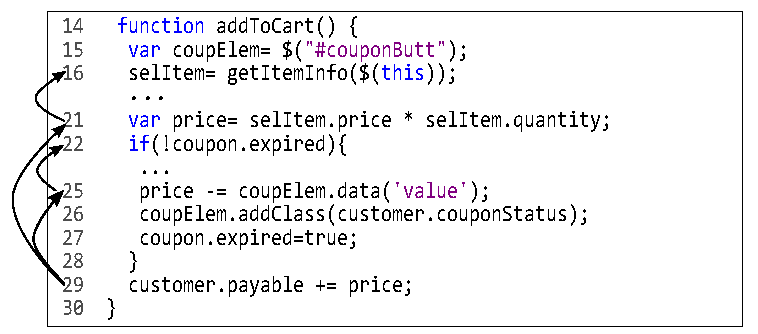
\includegraphics[width=1\hsize]{fig/intraCodeDep}
  \vspace{-0.3in} 
  \mycaption{Intra (data and control) code dependency through backward slicing.}
  \label{Fig:intraCodeDep}
  \vspace{-0.2in} 
\end{figure}
To determine the initial point of contact between DOM and the underlying application's code, we first cross reference the DOM element as well as the property we are interested in with a set of DOM mutations obtained from the execution trace. The desired DOM element and its property are inferred from either the intra DOM assertion dependency or the candidate DOM properties as described in \secref{extractDomRelatedInfo}. Recall that our execution trace contains information about triggered events, event handlers, and DOM mutations caused by the events. Therefore, we can identify relevant events and invoked functions corresponding to a given DOM mutation.
For example, the collected execution trace in \figref{assertionToCode} contains information about the mutations of a \code{div} element with class \code{shopContainer}, which pertains to the DOM-based assertion.

To figure out where the mutation originated in our execution trace, we keep record of DOM accesses within the invoked functions. For each DOM access, we track \javascript lines of code that are responsible for updating the corresponding DOM element. Going back to our example in \figref{assertionToCode}, given that the textual property of the \code{div} element is extracted from the intra DOM assertion dependency, we identify line 30 in function \code{viewCart} as the initial point of contact responsible for changing the \code{text} of DOM element.

After inferring DOM mutant statements, we identify the control and data \emph{intra code dependency} within the application's code.
%gather the entire set of \javascript statements responsible for mutating a given DOM element.
\begin{mydef}[Intra Code Dependency]
\label{def:intraCodeDep} 
 
An intra code dependency is defined as $<criterion, codeSts>$, where $criterion$ is a variable at the initial point of contact, and $codeSts$ is the set of control and data dependent statements that are either affected by the $ctiterion$ or have some effect on the $criterion$. 
\end{mydef}

To find the intra code dependency, we perform backward as well as forward slicing by using $criterion$ as the slicing criterion.
\textsc{GetBWSlice} in lines  15 and 21 of \algref{algorithm} computes a backward slice with respect to assertion related DOM mutations, and candidate DOM property mutations respectively.
We use dynamic slicing to capture run-time dependencies.
Note that instrumenting the entire application's code to perform dynamic slicing incurs high performance overheads. To avoid high overheads, we first intercept the code sent from the server to the client, and then statically instrument only those statements that may affect a given DOM element.
To extract the subset of the code statements, we first find the \javascript closure scope which contains the definition of the variable in the initial slicing criteria. Then all references to the variable within the closure scope are found. Therefore, we can identify all locations in the code where the variable is updated, read, or a new alias is created. For each variable update/read related to the variable of the slicing criteria, we track the data dependencies for such an operation. The aforementioned steps are performed iteratively for each dependencies to collect the subset of code statements, which are instrumented for a given initial slicing criteria.
The instrumented code keeps track of all updates and accesses to all relevant data and control dependencies.   
Once the test case runs, we collect traces from the instrumented code. This trace is used to dynamically extract backward slicing as well as forward slicing statements. Note that in addition to backwards slicing which is later used to generate explicit assertions, we also use forward slicing to generate our implicit assertions (\secref{implicitAssertions}).  

The backward slicing technique starts by extracting instances of the initial slicing criteria from the trace. For each \textit{read} operations, the trace is traversed backwards to find the nearest related \textit{write} operation. Once found, the \textit{write} operation is added to the slice under construction. This process is repeated for all the data dependencies related to that write operation. A similar approach is taken for including control dependencies in the slice. 
Our slicing technique supports inter-procedural slicing. For example, if a variable is assigned by the return value of a called function, the slicer recursively tracks the function and performs a backward slice on the statement returned by the called function.
%We track the following types of function calls during the slicing process: (1) Regular function calls e.g. \code{func()}, (2) Method calls e.g. \code{obj.func()}, (3) Constructors e.g. \code{new func()}, (4) Function handlers e.g. \code{element.click(func)}, and (5) Anonymous functions, which are assigned to a variable or an object property.
  
To address aliasing when computing the slice of a variable that has been set by a non-primitive value, we need to consider possible aliases that may refer to the same object. Specifically in \javascript \textit{dot notation} and \textit{bracket notation} are frequently used to modify objects at run time. Since static analysis techniques for \javascript often ignore this issue \cite{Feldthaus:icse13}, we use dynamic slicing. If a reference to an object of interest is saved to a second object's property, e.g. through the use of the \textit{dot notation}, the object of interest may also be altered via aliases of the second object. For example, after executing statement \code{a.b.c = objOfInterest;}, updates to \code{objOfInterest} may be possible through \code{a}, \code{a.b}, or \code{a.b.c}. To deal with such scenarios, our slicing technique searches through the collected trace and adds the forward slice for each detected alias to the current slice for our variable of interest (e.g. \code{objOfInterest}). 

Given \code{customer.payable} as the initial slicing criteria in our example, \figref{intraCodeDep} shows the relevant backward slice statements (lines 22, 18, 15, 14, and 9), where \code{customer.payable},  variable \code{price}, as well as properties of the object \code{selItem} are assigned, and the value of \code{coupon.expired} is checked in the conditional statement.
By the end of backward slicing step, we have all the relevant statements corresponding to a given DOM element. These are later used to derive test assertions.    
\subsection{Generating Unit-Level Assertions} \label{Sec:unitLevelAssertion}
Our approach targets postcondition assertions which are used to examine the expected behaviour of a given function after it is executed in a unit test case.
Through analyzing a given DOM-based test case, we generate unit-level assertions in the following three categories: (1) assertions, which are directly related to a given DOM-based assertion, (2) assertions, which are indirectly affected by a given DOM-based assertion, and (3) assertions that have direct impact on important DOM elements which are not checked by the existing DOM-based assertions. Each assertion is coupled with the expected value obtained from the execution trace of the application. The first type of assertion (type 1), which we call explicit assertion, can potentially be used in unit testing of the current version of the application. Type 2 and type 3, which we call implicit assertions and candidate assertions respectively, can be used for the purpose of regression testing.
\subsubsection{Explicit Assertions} \label{Sec:explicitAssertions}
After collecting all the statements, that are relevant to a given DOM-based assertion, we extract accessible entities from these statements (\textsc{Accessibles} in line 23 of the algorithm).
Types of accessible entities include (1) the function's returned value, (2) the used global variables in that function, (3) the object's property where the object is accessible in the outer scope of the function, and/or (4) the accessed DOM element in that function. Dynamic backward slice of a DOM-based assertion helps to (1) track all statements that contribute to the checked result and as such identify those entities that might have influenced the checked property value of the DOM element, and (2) eliminate unrelated entities that are not involved in the computation that leads to the update performed on the checked DOM element.

Since our dynamic slice is extracted from the program run, we can track all concrete values associated with accessible entities.
During the run of a test case, there might be different instances where a given statement is executed. Different execution instances can lead to different behaviour. Since we are using dynamic slicing, an instance that leads to the required behaviour, which is checked through the DOM-based assertion, is on the backward slice. Given that the manually-written expected value, that is checked against the DOM's property is valid, the concrete values of related entities in the backward slice are potentially correct. Therefore, concrete value of an entity in the backward slice can be used as the expected value of the entity in unit-level assertions to test the current version of the application (discussed in \secref{discussion}).
$explicitAsstn$ in line 23 of \algref{algorithm} contains the inferred explicit assertions.

In our running example (\figref{intraCodeDep}), explicit assertions check the correctness of \code{customer.payable}, \code{coupon.expired}, as well as \code{price} and \code{quantity} properties which belong to \code{selItem} object.
Assuming that the original price of the item is 100, the number of selected item is 1, and the calculated discount according to the \code{value} attribute of a DOM element with ID \code{couponButt} is 30, then the expected values included in the assertions for each of the entities are 70, boolean value \code{true}, 100, and 1, respectively. \figref{unitTest} shows a unit test case for \code{addToCart} function with the generated assertions in \qunit framework. %\karthik{What's a \qunit test?} 
Lines 7 to 9 in the figure corresponds to the explicit assertions.
\begin{figure}
  \centering
  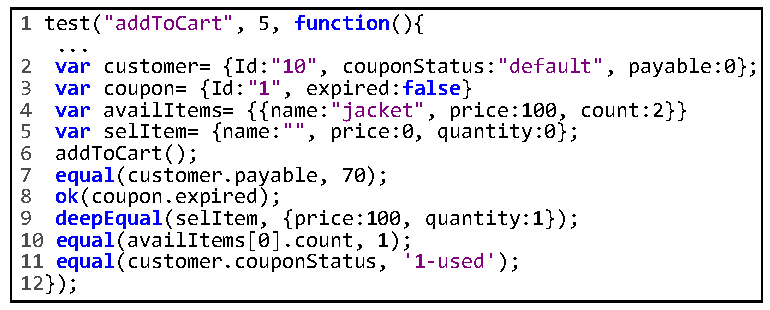
\includegraphics[width=1\hsize]{fig/unitTest}
   \vspace{-0.3in} 
  \mycaption{Generated \qunit test case and assertions.}
  \label{Fig:unitTest}
  \vspace{-0.28in} 
\end{figure}  
%We compare the value of the entity immediately after the relevant statement is executed in the backward slice with the entity's value before the function exits. If value of the entity remains the same, we use it towards the expected value in the unit-level assertion.  
%However, if the entity pertaining to a DOM change is reassigned in the code after the DOM gets updated and before the function exits, then the concrete value of the entity can be used for the purpose of regression testing unless the tester provides the proper expected value.
\subsubsection{Implicit Assertions} \label{Sec:implicitAssertions}
To this end we gather all the statements that explicitly affect the computations relevant to a given DOM-based assertion. While assertions inferred from such statements are inherently important, we further need to consider entities that are implicitly influenced by the checked DOM element in the manually-written test suite. For this purpose we apply a dynamic forward slice on the statements collected from a backward slice of a DOM-based assertion. A forward slice with respect to a statement $st$,
indicates how subsequently an operand at $st$ is being used. This can help the tester to ensure that $st$ properly establishes the expected outcome of the computations assumed by the later statements. 
Given the importance of statements involved in code-level computations of a DOM-based assertion, using forward slice is useful to check that there are no unforeseen effects on the application's behavior by a modification to such statements. 

Dynamic forward slice is performed on the subset of code statements which is previously instrumented as explained in \secref{domToCode}. The process of forwards slicing is similar to the backwards slicing technique as discussed earlier (\secref{domToCode}). The only difference is that it is performed in a forward direction. The slicing criterion of the forward slice module is either a variable, object's property, or an accessed DOM property extracted from the statements in a backward slice. The accessible entities, which have been set within the collected forward slice statements establish our implicit assertions.   
\subsubsection{Candidate Assertions} \label{Sec:candidateAssertions}
In addition to explicit and implicit assertions, we also verify the correctness of code-level entities pertaining to DOM updates, which are essentially important but not checked in the existing DOM-based test cases. We derive such unit-level assertions, namely candidate assertions, from the candidate DOM element properties previously obtained from the test case execution (box 3 in \figref{approachDiagram}). As the test case runs, we monitor DOM's evolution and match the list of mutated DOM elements and their properties with property updates of the candidate DOM elements. Once a match is found, we infer backwards slice statements pertaining to the mutation of DOM element's property (\textsc{GetBWSlice} in line 18 of the algorithm). Therefore, in this case the slicing criteria which is given as input to the backwards slicing module is an update to the property of the candidate DOM element.
After gathering the related \javascript statements within the application, we extract accessible entities of these statements (\textsc{Accessibles} in line 22) which form our candidate assertions. $candidateAsstn$ in line 22 contains our candidate assertions. 

Recall from the example (\figref{example}), one such potential DOM property which we record as part of \secref{extractDomRelatedInfo}, is \code{class} attribute associated with DOM element with ID \code{couponButt}. Monitoring DOM changes reveal that line 26, where the \code{class} attribute of the element is set, is the initial point of contact between DOM mutation and the \javascript code. Given line 26 as the slicing criteria, \code{customer.couponStatus} (line 24) is marked as the candidate assertion.
          
%mutation of customer.couponStatus = coupon.Id + '-' + 'used' to customer.couponStatus = coupon.Id + 'used';'